\section{Methods}
\subsection{Summary of the immersed boundary method}

Consider a $d$-dimensional ($d=2$ or 3) rectangular domain $\Omega$, which is
filled with a viscous incompressible fluid with constant viscosity $\mu$ and
density $\rho$, and contains an immersed elastic structure, $\Gamma$. The
structure is impermeable to the fluid and moves at the local fluid velocity, is
deformed by this motion, and imparts a force on the fluid. Otherwise, the
interface is treated as part of the fluid. 

The fluid velocity, $\vec{u} = \vec{u}(\vec{x},\,t)$, is governed by the
incompressible Navier-Stokes equations for a Newtonian fluid,
\begin{gather}
    \label{eq:ins-momentum}
    \rho(\vec{u}_t + \vec{u}\cdot\grad\vec{u}) = \mu\Delta\vec{u} - \grad p + \vec{f}, \\
    \label{eq:ins-incompressibility}
    \grad\cdot\vec{u} = 0,
\end{gather}
where $p$ is the hydrostatic pressure and $\vec{f}$ is the elastic force
density. This is a set of $d+1$ equations in $d+1$ unknowns: the $d$ components
of $\vec{u}$, and $p$. The equations are written relative to the Eulerian
frame, so that the coordinates $\vec{x}$ are independent variables. Quantities
in the Eulerian frame are written in the lower case Latin alphabet.

Let $\vec{X}=\vec{X}(\vec{\theta},\,t)$ represent a parametrization of the
Cartesian coordinates of an immersed interface with material coordinates
$\vec{\theta}$ at time $t$. Let $\mathcal{E}[\vec{X}]$ be the energy density
functional for the elastic interface material. The elastic force density is
computed by evaluating the Fréchet derivative of $\mathcal{E}$,
\begin{equation}
    \vec{F} = -\delta \mathcal{E}[\vec{X}],
\end{equation}
where $\delta$ represents the first variation. Upper case Latin letters
represent Lagrangian quantities and are functions of $\vec{\theta}$ and $t$.

To couple the fluid and interface, we employ the Dirac delta function,
$\delta(\vec{x}-\vec{X}(\vec{\theta},\,t))$. Analytically, the fluid-interface
interactions can be written
\begin{gather}
    \label{eq:interpolation}
    \dot{\vec{X}} = \int_\Omega \delta(\vec{x}-\vec{X}) \vec{u}(\vec{x},\,t)\d\vec{x},\ \text{and} \\
    \label{eq:spreading}
    \vec{f} = \int_\Gamma \delta(\vec{x}-\vec{X})\vec{F}(\vec{X})\d\vec{X},
\end{gather}
where $\dot{\vec{X}}$ represents the derivative of $\vec{X}$ with respect to
$t$. [@eq:interpolation] is called interpolation, and the result of the
right-hand side is the fluid velocity at $\vec{X}$; namely, $\dot{\vec{X}}
= \vec{u}(\vec{X},\,t)$. [@eq:spreading] is called spreading, because while
$\vec{F}$ has units of force per unit \emph{area} on $\Gamma$, $\vec{f}$ has
units of force per unit \emph{volume} in $\Omega$. The force $\vec{F}\d\vec{X}$
over area $\d\vec{X}$ is "spread" to the force $\vec{f}\d\vec{x}$ over volume
$\d\vec{x}$. 

Each of the fluid equations is discretized on a regular grid of spacing $h$ so
that $\Omega$ is divided into cubic cells of side length $h$. The grids can be
collocated or staggered. Because of the checkerboard instability (see, e.g.,
[@Wesseling:2001ci]) in solving the Navier-Stokes equations on collocated
regular grids, we will assume that the grids are staggered. This means that
different components of a single Eulerian vector quantity, such as $\vec{u}$,
might be evaluated at different locations. However, corresponding components of
vector-valued Eulerian quantities, and those of $\vec{u}$ and $\vec{f}$ in
particular, are assumed to be discretized on the same grid. A fixed Lagrangian
point may reside in different grid cells for each different grid. The set of
Eulerian grid points for a grid will be denoted $\Omega^h$, and define
$n_\omega = |\Omega^h|$.

The Lagrangian force density $\vec{F}$ is evaluated at a set of points,
usually a \emph{fixed} set of points in the Lagrangian variables,
$\vec{\theta}$.  The notation $\vec{X}_j=\vec{X}(\vec{\theta}_j,\,t)$ refers to
an individual Lagrangian point. The typical heuristic for distributing the
points $\vec{X}_j$ on the elastic interface is that neighboring Lagrangian
points be at most $h$ apart from one another, and often at most $h/2$ apart. We
denote the set of Lagrangian points by $\Gamma^h$ and define $n_\gamma =
|\Gamma^h|$ to be the number of Lagrangian points.

\begin{figure}[thb]
    \centering
    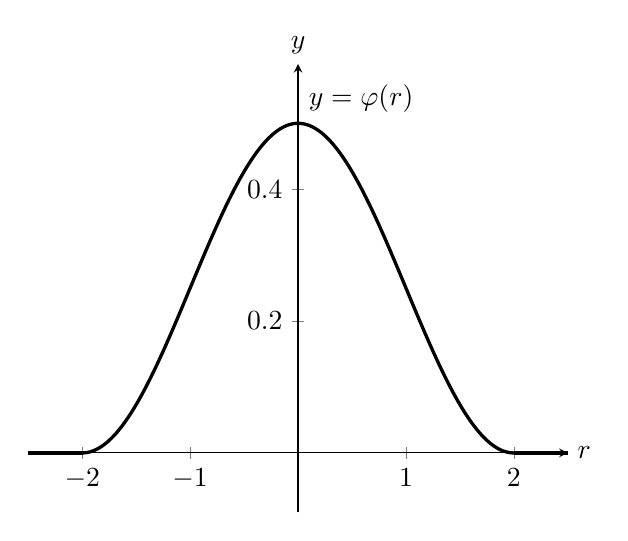
\begin{tikzpicture}
        \begin{axis}[ymin=-0.09, ymax=0.59, xmin=-2.5, xmax=2.5, axis lines=center, xlabel={$r$}, ylabel={$y$}, xlabel style={right}, ylabel style={above}, smooth, no markers]
            \addplot[samples=400, domain=-2: 2, very thick, black] {0.25 * (1+cos(90*x))} node[midway, above right] {$y=\varphi(r)$};
            \addplot[samples=400, domain=-3:-2, very thick, black] {0};
            \addplot[samples=400, domain= 2: 3, very thick, black] {0};
        \end{axis}
    \end{tikzpicture}
    \caption{%
        A compactly-supported approximation to the Dirac delta function. The
        quantity $r$ is the difference in position of an Eulerian and
        a Lagrangian point in units of grid spaces. For $r\in[0,\,1)$, only
        $\varphi(r-2)$, $\varphi(r-1)$, $\varphi(r)$, and $\varphi(r+1)$ are
        nonzero for points spaced 1 apart.
    }
    \label{fig:1d-kernel}
\end{figure}

The singular [integrals @eq:interpolation;@eq:spreading] do not lend themselves
easily to evaluation. In particular, it is unlikely that Lagrangian points and
Eulerian grid points will coincide. For a regular grid with spacing $h$, we
replace the Dirac $\delta$-function with a regularized kernel, $\delta_h$,
which is a Cartesian product of one-dimensional kernels,
$h^{-1}\varphi(h^{-1}x)$. One choice for $\varphi$ is shown in [@fig:1d-kernel]. 

A single step of the IB method proceeds roughly as follows:
\begin{enumerate}[label=(\texttt{\alph*})]
    \item interpolate $\vec{u}^n$ to $\vec{X}^n$ to get $\vec{U}^\ast$,
    \item predict data site positions $\vec{X}^\ast = \vec{X}^n + \alpha k\vec{U}^\ast$,
    \item compute Lagrangian forces $\vec{F}^\ast$ using positions $\vec{X}^\ast$,
    \item spread $\vec{F}^\ast$ from $\vec{X}^\ast$ to get $\vec{f}^\ast$,
    \item solve for updated velocities $\vec{u}^\ast$,
    \item project $\vec{u}^\ast$ into space of divergence-free vector fields to
        get $\vec{u}^{n+1}$,
    \item interpolate $\vec{u}^{n}$ to $\vec{X}^{n}$ to get $\vec{U}^{n+1}$, and
    \item update $\vec{X}^{n+1} = \vec{X} + k \vec{U}^{n+1}$.
\end{enumerate}
We group these steps into 6 major operations: (1) velocity interpolation;
(2) cell update, which includes updating some geometric information; (3)
Lagrangian force computation; (4) force spread; (5) velocity update; and (6)
velocity field projection. The next section introduces some details for the
various immersed structures used in our simulations. The remainder of this
paper describes each of these operations in detail.

\subsection{Spatial discretization}

The equations [@eq:...] are discretized on staggered, regular grids with grid
spacing $h$. The components of vector-valued quantities are discretized on the
center of the corresponding cell face. That is, for example, if
$\vec{a} = (a_1,\,a_2,\,a_3)$ are the three components of a vector-valued
quantity for some grid cell with lower corner $h(i,\,j,\,k)$, then $a_1$
lives at $h(i,\,j+0.5,\,k+0.5)$, $a_2$ at $h(i+0.5,\,j,\,k+0.5)$, and $a_3$ at
$h(i+0.5,\,j+0.5,\,k)$. Scalar quantities are discretized at cell centers,
e.g., $h(i+0.5,\,j+0.5,\,k+0.5)$.

The central difference operator $D^i$, which differentiates with respect to
the $i^\text{th}$ coordinate, in the absence of solid boundaries, is defined as
\begin{equation}
    D_ig(\vec{x}) = \frac{g(\vec{x}+h\vec{e}_i/2) + g(\vec{x}+h\vec{e}_i/2)}{h}.
\end{equation}
In the presence of solid boundaries, a linear interpolant is used to fill a
ghost value. The divergence operator applied to a vector-valued function
$\vec{a}$ on the staggered grid, $\grad_h\cdot\vec{a} = D_ia^i$, where Einstein
summation notation is assumed and $i$ ranges from 1 to $d$, results in
a scalar-valued quantity at the cell center. The gradient operator applied to
scalar-valued quantity $b$ at the cell center yields the vector
$\grad_hb = \vec{e}^jD_jb$ on the staggered grid.

Define the central averaging operator, $A^i$, which averages in the
$i^\text{th}$ coordinate direction and in the absence of boundaries, as
\begin{equation}
    A_i = \frac{g(\vec{x}+h\vec{e}_i)+g(\vec{x}-h\vec{e}_i)}{2}.
\end{equation}
In the presence of boundaries, we use the value at the ghost cell. By taking
products of averaged components of $\vec{u}$, we compute advection in
conservation form as
\begin{equation}
    \vec{H}(\vec{u}) := \vec{e}_iD_j((\delta^{im}A_mu^j)(\delta^{jn}A_nu^i)).
\end{equation}

The viscous terms are computed as $\mu\Delta_h\vec{u}$, where $\Delta_h$ is the
standard 5- or 7-point Laplacian. In the absence of solid boundaries, this
is identical to  $\Delta_h = \grad_h\cdot\grad_h$. Otherwise, we use the value
at the ghost cell for stencils that extend past a solid boundary.

\subsection{Temporal discretization}

We time-step using the 2$^\text{nd}$ order implicit-explicit Runge-Kutta method
as described in [@Peskin:...] and projection method PmIII from [@Brown:...].
This leads to the system of equations
\begin{align}
    \left(\tilde{I}-\frac{\lambda}2\Delta_h\right)\delta\vec{w}
    &= \alpha\lambda\left[\Delta_h\vec{u}^n + B_h \vec{w}_b^{n+\sfrac12}\right] + \tilde{I}\left(\rho^{-1}\vec{f} - \vec{H}(\vec{u}^{n+\alpha-\sfrac12})\right) \\
    \vec{w} &= \vec{u}^n + \delta\vec{w} \\
    k\Delta_h\phi &= \grad_h\cdot\vec{w} \\
    \vec{u}^{n+\alpha} &= \vec{u}^\ast - k\grad_h\phi,
\end{align}
where $k$ is the timestep, $\lambda = k\mu/\rho$, $B_h$ is an appropriate
boundary operator for the discrete Laplacian, $\vec{w}_b$ are boundary data for
$\vec{w}$, and $\alpha$ is the fraction of the timestep for the current stage
of the timestepping method: $\alpha=\sfrac12$ or 1. The quantity $\phi$ acts as
a pseudo-pressure, and the pressure can be recovered via
$p=\phi-(\mu/\rho)\grad_h\cdot\vec{w}$.

The modified identity matrix, $\tilde{I}$, corrects errors in using the
standard discrete Laplacian on a staggered grid, where the stencil may extend
beyond the boundary of the domain. This requires a ghost point, to which we
have assigned a value using a linear interpolant. Under certain circumstances,
this works perfectly fine, but in general, the resulting approximation to the
Laplacian is 0$^\text{th}$ order, but differs by a constant factor. Let that
factor be denoted $1-\epsilon_h$. For stencils that straddle the boundary, we
modify the momentum equation so that we are instead solving
\begin{equation}
    (1-\epsilon_h)\rho(\vec{u}_t + \grad\cdot(\vec{u}\otimes\vec{u})) = (1-\epsilon_h)\left[\mu\Delta\vec{u} + \vec{f}\right].
\end{equation}
This requires no additional modification to the Laplacian, but after
discretization, yields a factor in front of the intermediate velocity update
$\delta\vec{w}$ and the force density and advection terms. Under reasonable
assumptions, the resulting linear system is symmetric positive definite, and
is suitable for use with preconditioned conjugate gradients. One can view this
as using a quadratic interpolant near the boundaries and scaling the
corresponding rows to ensure symmetry of the linear system. The resulting
systems are identical.

To solve the Helmholtz system $\tilde{I}-\sfrac12\lambda\Delta_h$, we use
conjugate gradients preconditioned with Chebyshev iteration. Chebyshev
iteration requires only that the matrix be positive (negative) semi-definite,
and uses only matrix-vector multiplication and vector scaling, it is
parallelizable if those two operations are. Vector scaling is trivially
parallelilzable, and for certain matrix formats, such as compressed sparse row,
matrix-vector multiplication is parallelizable as well.

Chebyshev iteration can also be modified for use as a smoother/relaxer for
multigrid. Its efficacy is comparable or better to that of successive
over-relaxation (SOR), but the parallelism of Chebyshev iteration far exceeds
that of SOR. To solve the Poisson problem for $\phi$, we employ multigrid with
a Chebyshev smoother as a preconditioner for conjugate gradients.


\subsection{Surface geometry via radial basis function interpolation}

Fix a set of distinct points $\{\vec{\theta}_i\}_{i=1}^{n_d}$ in parameter
space. We refer to these $n_d$ points as \textit{data sites} and are used to
construct an interpolant which will acts as the surface of a cell. To
accomplish this, we track the coordinates in $\mathbb{R}^3$ of the point on the
surface corresponding to each of the data sites.

We can choose a set of distinct points in parameter space, called the
\textit{sample sites}, which are possibly different from the data sites, at
which to evaluate the interpolant and its derivatives, and ultimately to
compute the Lagrangian force density. These points will be used to spread force
density from the surface to the Eulerian grid, so we choose them to satisfy the
IB method heuristic that the mesh size $h_s$ satisfies $h_s \lesssim h/2$,
where $h$ is the Eulerian grid size.

The surface interpolant is constructed from a linear combination of radial
basis functions and another polynomial basis. While generally, these basis
functions may not be true polynomials, we will refer to them as such for 
simplicity of illustration. Details ... [@Shankar:...].

Let $\vec{X}_k$ be the coordinates of the point on the cell surface
corresponding to data site $\vec{\theta}_k$. The interpolant should recover
these coordinates exactly, for each data site. In other words, we want
\begin{equation}
    \vec{X}_k = \sum_{i=1}^{n_d} b_i\varphi(d(\vec{\theta}_k,\,\vec{\theta}_i)) + \sum_{j=1}^{n_p} c_jp_j(\vec{\theta}_k),
\end{equation}
where $\varphi$ is called the \textit{basic function}, $d$ is a suitable metric
for the object under study, and $n_p$ is the number of elements in the set of
polynomial basis functions $\{p_j\}_{j=1}^{n_p}$. For certain choices of
$\varphi$, $n+p\ge 1$ may be required [@Wendland:...;@Fasshauer:...]. For an
individual component of $\vec{X}$ at each data site, this yields $n_d$
conditions in $n_d+n_p$ variables. To uniquely determine the interpolant, we
require further that the polynomial basis recover polynomial data:
\begin{equation}
    0 = \sum_{i=1}^{n_d} b_ip_j(\vec{\theta}_i).
\end{equation}
Collectively, these conditions can be written
\begin{equation}
    \label{eq:rbf-interpolant}
    \left[\begin{array}{cc}\Phi & P \\ P^T & 0\end{array}\right]
    \left[\begin{array}{c}\vec{b}\\\vec{c}\end{array}\right] =
    \left[\begin{array}{c}\vec{X}\\\vec{0}\end{array}\right].
\end{equation}
Assuming that the system is uniquely determined, we have constructed our
interpolant.

Let $\mathcal{L}$ be a linear operator for which $\Psi=(\mathcal{L}\varphi(d(\vec{\theta},\,\vec{\theta}_i)))$,
for $i=1,\,\ldots,\,n_d$, and $Q=(\mathcal{L}p_j(\vec{\theta}))$, for $j=1,\,\ldots,\,n_p$,
can be computed analytically. For the purposes of computing Lagrangian force
density, of particular interest are the identity (or "evaluation") operator,
and the various first and second partial derivative operators. With
a sufficiently smooth choice of $\varphi$, we can approximate $\mathcal{L}\vec{X}(\vec{\theta})$
at an arbitrary point in parameter space by applying the operator $\mathcal{L}$
to the interpolant and evaluating the result. That is,
\begin{equation}
    \mathcal{L}\vec{X}(\vec{\theta})
    \approx \sum_{i=1}^{n_d} b_i\mathcal{L}\varphi(d(\vec{\theta},\,\vec{\theta}_i))
    + \sum_{j=1}^{n_p} c_j\mathcal{L}p_j(\vec{\theta})
\end{equation}
by linearity. But the coefficients $\vec{b}$ and $\vec{c}$ are determined by
the interpolant [@eq:rbf-interpolant], so
\begin{align}
    \mathcal{L}\vec{X}(\vec{\theta})
    &= \left[\begin{array}{cc}\Psi&Q\end{array}\right]
    \left[\begin{array}{cc}\Phi&P\\P^T&0\end{array}\right]
    \left[\begin{array}{c}\vec{X}\\\vec{0}\end{array}\right] \\
    &= \left[\begin{array}{cc}L&\ast\end{array}\right]
    \left[\begin{array}{c}\vec{X}\\\vec{0}\end{array}\right],
\end{align}
where $L\vec{X}$ is now the discrete analogue to $\mathcal{L}\vec{X}(\vec{\theta})$,
i.e., the operator that applies $\mathcal{L}$ and evaluates at $\vec{\theta}$.
The $n_p$ columns represented by $\ast$ are usually ignored, as they are
always multiplied by a vector of zeros and therefore do not contribute.

We also require integration weights, which act as surface patch areas in
computing surface forces from a surface force density. In many cases, the
integral
\begin{equation}
    I_\varphi(\vec{\theta}') = \int_\Gamma \varphi(d(\vec{\theta},\,\vec{\theta}'))\mskip\thinmuskip\mathrm{d}\hat{\vec{X}}(\vec{\theta})
\end{equation}
may not be known for topological archetype $\Gamma$. But
following the work of [@Narcowitz:...], for certain surfaces,
$I_\varphi(\vec{\theta}')$ is independent of $\vec{\theta}'$ and is therefore
constant. Assuming $I_\varphi = \text{constant}$ and
\begin{equation}
    I_1 = \int_\Gamma \mathrm{d}\hat{\vec{X}}(\vec{\theta})
\end{equation}
is known, we can compute integration weights $\hat{\vec{a}}$ for $\Gamma$ via
\begin{equation}
    \left[\begin{array}{cc}\Phi &\vec{1} \\ \vec{1}^T & 0\end{array}\right]
    \left[\begin{array}{c}\hat{\vec{a}}\\-I_\varphi\end{array}\right] =
    \left[\begin{array}{c}\vec{0}\\I_1\end{array}\right].
\end{equation}
A side effect of solving this system is that we obtain an approximation to
the constant $I_\varphi$.

To compute integration weights for a shape $\vec{X}(\vec{\theta})$, which is
topologically equivalent to $\hat{\Gamma}$, we compute the
Jacobian for $\hat{\Gamma}$ and the cell,
\begin{equation}
    \hat{V}=\left|\frac{\partial\hat{\vec{X}}}{\partial\theta^i}\right| \quad \text{and} \quad
    V=\left|\frac{\partial\vec{X}}{\partial\theta^i}\right|.
\end{equation}
Since $\hat{\Gamma}$ is known, we can compute $\hat{V}$ analytically. The
expression $a_k/\hat{V}(\vec{\theta}_k)$ gives the integration weight in
parameter space and can be computed without any information about the cell,
except that the cell and $\Gamma$ are topologically equivalent. From these
weights and an interpolant for the cell, the expression
$\mathrm{d}A_k=a_k V(\vec{\theta}_k)/\hat{V}(\vec{\theta}_k)$ gives the
integration weight on the surface of the cell.


\subsection{Computation of Lagrangian forces}

To compute forces for a cell, we follow the analysis of [@Maxian:...]. The
constitutive laws of interest for our purposes are the Skalak tension law,
\begin{equation}
    W_\text{Sk} = \frac{G}{4}(I_1^2-2I_1+2I_2) + \frac{K}{4}I_2^2;
\end{equation}
the neo-Hookean tension model,
\begin{equation}
    W_\text{nH} = \frac{G}{2}\left(\frac{I_1+2}{\sqrt{I_2+1}}-1\right) + \frac{K}{2}\left(\sqrt{I_1+1}-1\right)^2;
\end{equation}
Hookean tether energy,
\begin{equation}
    W_\text{tether} = \frac{k}{2}\|\vec{X}-\vec{Z}\|^2;
\end{equation}
and the Canham-Helfrich bending energy,
\begin{equation}
    W_\text{CH} = \frac{\kappa}{2}(H-H_0)^2.
\end{equation}
In the above, $G$, $K$, and $\kappa$ are the shear, bulk, and bending moduli,
respectively; $k$ is the spring constant; and $H_0$ is the preferred mean
curvature of the surface.

For each of these, we can compute analytically the force density by directly
computing the first variation of the energy functional
\begin{equation}
    \mathcal{E}[\vec{X}] = \int_\Gamma W\mskip\thinmuskip\mathrm{d}\vec{X}.
\end{equation}
For the Skalak and neo-Hookean tension models, we can rewrite the energy
functional in terms of the undeformed configurations, and write the force
density as
\begin{equation}
    \vec{F} = \frac{1}{\sqrt{\hat{g}}}\frac{\partial}{\partial\theta^j}\left(\sqrt{\hat{g}}\left[\Phi \hat{g}^{ij} + I_2\Psi g^{ij}\right]\frac{\partial\vec{X}}{\partial\theta^i}\right),
\end{equation}
were $\hat{g}^{ij}$ and $\hat{g}$ are the inverse and determinant of the metric
tensor
\begin{equation}
    g_{ij} = \frac{\partial\hat{\vec{X}}}{\partial\theta^i}\cdot\frac{\partial\hat{\vec{X}}}{\partial\theta^j},
\end{equation}
respectively. The inverse metric tensor $g^{ij}$ is the analogue of $\hat{g}^{ij}$
for the deformed configuration. The material functions $\Phi$ and $\Psi$ are
the partial derivatives of the constitutive law, $W$, with respect to $I_1$
and $I_2$, respectively, and the bracketed terms are also known as the
second Piola-Kirchhoff stress tensor. The tether energy yields the tether
force density
\begin{equation}
    \vec{F}_\text{tether} = -k(\vec{X}-\hat{\vec{X}}),
\end{equation}
and the Canham-Helfrich bending energy yields the bending force density
\begin{equation}
\vec{F}_\text{tether} = -\kappa\left[\Delta_{\vec{\theta}}(H-H_0) + (H-H_0)(2H^2-\mathcal{R})\right]\vec{n},
\end{equation}
where, $\mathcal{R}$ is the scalar curvature of the deformed configuration.


\subsection{Parallelization of interaction operators}

Below, we describe a method for evaluating
\begin{align}
    \label{eq:scalar-interp}
    E(\vec{X}) &= \int_\Omega \delta_h(\vec{x}-\vec{X})e(\vec{x}) \d\omega \quad \text{and}\\
    \label{eq:scalar-spread}
    \ell(\vec{x}) &= \int_\Gamma \delta_h(\vec{x}-\vec{X})L(\vec{X}) \d\gamma
\end{align}
for scalar-valued functions $e: \Omega\to\mathbb{R}$ and $L:\Gamma\to\mathbb{R}$.
For vector-valued functions, such as $\vec{u}$ and $\vec{F}$, the algorithm
can be applied to each component individually. For some grids, it may be
possible to process each component concurrently. We consider this possibility
at the end of the section.

\subsection{The structure of $\mathcal{S}$ and $\mathcal{S}^\dagger$}

Let $\Omega_h$ be a regular grid on $\Omega$ with grid spacing $h$. Define
$\vec{g} \in [0,\,1)^d$ to be the fixed vector such that a grid point $\vec{x}$
can be decomposed as $\vec{x}=h(\vec{i}+\vec{g})$, where $\vec{i}$ has integer
components. Moreover, let $\Gamma_h$ be a discretization of the interface
$\Gamma$. For illustration purposes, we can think of $\Gamma_h$ as a collection
of arbitrary points in $\Omega$. We refer to points in $\Omega_h$ as (Eulerian)
grid ponts, and points in $\Gamma_h$ as Lagrangian points.

[Equations @eq:scalar-interp;@eq:scalar-spread] are discretized on $\Omega_h$
and $\Gamma_h$, respectively, to yield
\begin{align}
    \label{eq:disc-interp}
    E(\vec{X}_j) &= \sum_i \delta_h(\vec{x}_i-\vec{X}_j)e(\vec{x}_i) h^d \quad \text{and} \\
    \label{eq:disc-spread}
    \ell(\vec{x}_i) &= \sum_j \delta_h(\vec{x}_i-\vec{X}_j)L(\vec{X}_j) \d A.
\end{align}
Each of the above equations look like a matrix-vector multiplication, so we 
will define $\mathcal{S}=(\delta_h(\vec{x}_i-\vec{X}_j))$, where the subscript
$i$ indicates the row and subscript $j$ indicates the column. Collecting the
values of $e(\vec{x})$ at each Eulerian grid point and of $L(\vec{X})$ at
each Lagrangian point, we rewrite [equations @eq:disc-interp;@eq:disc-spread]
as
\begin{align}
    \label{eq:matrix-interp}
    \vec{E} &= \mathcal{S}^\dagger\vec{e} \quad\text{and} \\
    \label{eq:matrix-spread}
    \vec{\ell} &= \mathcal{S}\vec{L},
\end{align}
respectively. For this reason, we call $\mathcal{S}$ the \emph{spread matrix},
and its transpose, $\mathcal{S}^\dagger$, the \emph{interpolation matrix}.

As we have said, $\delta_h$ is the tensor product of scaled, one-dimensional
kernels, $h^{-1}\phi(h^{-1}x)$. Let $\mathrm{supp}\mskip\thinmuskip\phi$
denote the support of $\phi$ and define
\begin{equation}
    s[\phi] = |\mathrm{supp}\mskip\thinmuskip\phi\cap\mathbb{Z}|-1
\end{equation}
to be the size of the support in meshwidths. For brevity, we write $s=s[\phi]$.
For any $\vec{X}\in\Omega$, there are at most $s^d$ grid points
$\vec{x}\in\Omega_h$ for which $\delta_h(\vec{x}-\vec{X})$ is nonzero.

Let $\vec{y}\in\Omega$ be an arbitrary point and consider the set of grid
points for which $\delta_h(\vec{x}-\vec{y})$ and $\vec{x}\in\Omega_h$. Denote
this set of grid points $\Sigma(\vec{y})$, called the \emph{support points}
of $\vec{y}$. The pre-image $\Sigma^{-1}(\Sigma(\vec{y}))$ is a subset of
$\Omega$ containing at most one grid point. For $\vec{y}$ sufficiently far away
from any boundary, $\Sigma^{-1}(\Sigma(\vec{y}))$ is an $h \times h$ ($d=2$) or
$h \times h \times h$ ($d=3$) subset of $\Omega$. For points near a boundary,
the region may be smaller. Collectively, these regions cover $\Omega$, so we
consider them to be the \emph{de facto} grid cells. For those grid cells that
do not contain a grid point, we extend $\Omega_h$, in a regular way, with ghost
points. Call this extension $\bar{\Omega}_h$. Now, any $h \times h$ or
$h \times h \times h$ extended grid cell that entirely contains a grid cell
also contains exactly one grid point in $\bar{\Omega}_h$, including grid cells
near a boundary. We can identify an $\vec{y}\in\Omega$ with a grid point
$\vec{x}\in\bar{\Omega}_h$ if they are in the same extended grid cell, and
since $\vec{x}=h(\vec{i}=\vec{g})$, we identify a grid cell by the integers
$\vec{i}$. Finally, we define $\lfloor\cdot\rceil:\Omega\to\mathbb{Z}$ such
that $\lfloor\vec{y}\rceil = \vec{i}$.

We now turn our attention to the evaluation of $\delta_h(\vec{x}-\vec{X})$. We
assume $\vec{x}\in\Omega_h$ and write
\begin{equation}
    \label{eq:delta-defs}
    \begin{aligned}
        \delta_h(\vec{x}-\vec{X})
        &= \delta_h(\vec{x}-h(\lfloor\vec{X}\rceil+\vec{g}) + h(\lfloor\vec{X}\rceil+\vec{g}) - \vec{X}) \\
        &= \delta_h(h\vec{\sigma} - \Delta\vec{X}) \\
        &= \prod_{i=1}^d h^{-1}\phi((\vec{\sigma} - h^{-1}\Delta\vec{X})\cdot\vec{c}_i).
    \end{aligned}
\end{equation}
where $\Delta\vec{X}$ is the displacement of $\vec{X}$ from its associated grid
point, $\vec{\sigma} = \lfloor\vec{x}\rceil-\lfloor\vec{X}\rceil$ since
$\vec{x} = h(\lfloor\vec{x}\rceil+\vec{g})$, and $\vec{c}_i$ is the $i^\text{th}$
canonical basis vector. We refer to $\vec{\sigma}$ as a \emph{shift}. Shifts
that result in a possibly nonzero value of $\delta_h$ are known \emph{a priori}
based on $\phi$, and usually range from $-\lfloor s/2\rfloor$ to
$\lfloor(s-1)/2\rfloor$ in each component. We can therefore choose an order for
the shifts $\{\vec{\sigma}_i\}_{i=1}^{s^d}$. We denote the $i^\text{th}$ shift
$\vec{\sigma}_i$.

We need one more ingredient to construct $\mathcal{S}$. Let $\vec{x}_k$ be the
be the $k^\text{th}$ grid point, such that, e.g., $e_k = e(\vec{x}_k)$ is the $k^\text{th}$
entry of $\vec{e}$. The grid point $\vec{x}_k$ can be decomposed into
$h(\vec{i}+\vec{g})$ for some $\vec{i}$ with integer components. Define the
grid indexing function $\#:\mathbb{Z}^d\to\mathbb{Z}\cup\{\epsilon\}$ such that
$\#(\lfloor\vec{x}_k\rceil) = \#(\vec{i}) = k$ for all grid points and
$\#(\vec{i}')=\epsilon$ if $h(\vec{i}'+\vec{g}) \not\in \Omega$.

We are now ready to construct $\mathcal{S}$. Consider a Lagrangian point
$\vec{X}_j$ that is in the same grid cell as grid point
$\vec{x}_k=h(\lfloor\vec{X}_j\rceil+\vec{g})$. The $j^\text{th}$ column of
$\mathcal{S}$ is zero except for up to $s^d$ values where for
$i=1,\,\ldots,\,s^d$, if $\#(\lfloor\vec{X}_j\rceil+\vec{\sigma}_i)\neq\epsilon$,
\begin{equation}
    \label{eq:s-columnwise}
    \mathcal{S}_{i,\#(\lfloor\vec{X}_j\rceil + \vec{\sigma}_i)} = \delta_h(h\vec{\sigma}_i-\vec{X}_j+\vec{x}_k).
\end{equation}

\subsection{Parallelization of interpolation}
From the above, we can see that $\mathcal{S}$ has approximately equal number
of nonzero entries per column. This means, that the interpolation matrix,
$\mathcal{S}^\dagger$, has approximately equal number of nonzero entries per row.
This property is beneficial for parallelization. Consider the $j^\text{th}$ row of
$\mathcal{S}^\dagger$, which corresponds to interpolating to Lagrangian point
$\vec{X}_j$ using the values at its support points. There are at most $s^d$
values in that row, which correspond to the shifts that give a potentially
nonzero value for $\delta_h$. Compute $\vec{x} = h(\lfloor\vec{X}_j\rceil+\vec{g})$.
Then $\Delta\vec{X} = \vec{X}_j-\vec{x}$. Now, since the shifts $\{\vec{\sigma}_i\}$
are known beforehand, we can compute $\delta_h(\vec{\sigma}_i-\Delta\vec{X})$
and, if $\#(\vec{\sigma}_i+\lfloor\vec{x}\rceil) \neq\epsilon$, we accumulate
products
\begin{equation*}
    E_j = \sum_{i=1}^{s^d}\delta_h(\vec{\sigma}_i+\Delta\vec{X})e_{\#(\vec{\sigma}_i+\lfloor\vec{x}\rceil)}.
\end{equation*}

Assigning one thread per Lagrangian point (i.e., one thread per row), this
calculation can be performed in parallel, and since the $j^\text{th}$ thread writes
to the $j^\text{th}$ entry of $\vec{E}$, there are no write contentions. Because the
number of products is approximately the same for each row, each thread does
approximately the same amount of work. On architectures that enforce thread
synchrony, such as GPUs, this means that we do not incur a penalty from having
threads wait for other threads to finish.

Since each thread computes the appropriate $\delta_h$-weights for its own row,
it is unnecessary to construct $\mathcal{S}^\dagger$ explicitly. Other than
allocating memory for $\vec{E}$, all of the work for this algorithm is parallel,
so we expect to see near-perfect scaling and a theoretical runtime of
$\mathcal{O}(n_\gamma/p)$, where $p$ is the number of threads.

\subsection{Parallelization of spread}
The difficulty arises in attempting to parallelize the spread operation.
Row-wise parallelization of $\mathcal{S}\vec{L}$ yields threads doing vastly
different amounts of work -- many no work at all -- and incurring the penalty
of having threads wait for other threads to finish before being able to
continue. Moreover, this parallelization would scale according to the size of
the Eulerian grid rather than the number of Lagrangian points.

Instead, we wish to partition the work so that every thread does a similar
amount of work, it scales well, and depends minimally on the size of the
background grid. We can think of this as finding matrices $\mathcal{S}_1$,
$\mathcal{S}_2$, \dots, $\mathcal{S}_m$ and vectors $\vec{L}_1$, $\vec{L}_2$,
\dots, $\vec{L}_m$ such that
\begin{equation*}
    \vec{\ell} = \mathcal{S}\vec{L} = \mathcal{S}_1\vec{L}_1 + \mathcal{S}_2\vec{L}_2 + \cdots + \mathcal{S}_m\vec{L}_m.
\end{equation*}
Here, $m$ is the number of serial operations or \emph{sweeps} needed to
completely compute $\mathcal{S}\vec{L}$. The products $\mathcal{S}_i\vec{L}_i$
are accumulated serially, but we aim to construct the matrices
$\{\mathcal{S}_i\}$ in a way that allows for efficient parallel computation of
each individual product.

Consider two points in different grid cells, $\vec{x}_1$ and $\vec{x}_2$. Since
these points are in different grid cells, the support points
$h(\lfloor\vec{x}_1\rceil+\vec{g}+\vec{\sigma}_i)$ of $\vec{x}_1$ and 
$h(\lfloor\vec{x}_2\rceil+\vec{g}+\vec{\sigma}_i)$ of $\vec{x}_2$, assuming
they exist, are distinct for $i=1,\,\ldots,\,s^d$. Thus, for any set
$\{\vec{X}_j\}$ of Lagrangian points, each in different grid cells, the values
\begin{equation*}
    \delta_h(h(\lfloor\vec{X}_j\rceil + \vec{g}+\vec{\sigma}_i)-\vec{X}_j)L_j,
\end{equation*}
for $\#(\lfloor\vec{X}_j\rceil+\vec{\sigma}_i)\neq\epsilon$, can be computed
and written in parallel for fixed $i$, because the values of
$\#(\lfloor\vec{X}_j\rceil+\vec{\sigma}_i)$, when not equal to $\epsilon$, are
distinct, and gives the index of the output entry of $\vec{\ell}$.
Repeating for $i=1,\,\ldots,\,s^d$, we compute all of $\vec{\ell}$.

Consider now a set of Lagrangian points $\{\vec{X}_j\}$ all in the same grid
cell. For fixed $i$, the values $\#(\lfloor\vec{X}_j\rceil+\vec{\sigma}_i)$ are
identical for all $j$, and would therefore contend with one another if
attempting to write values in parallel and independently. In this case, we
can use the well-know parallel reduce algorithm to accumulate values in
parallel and ultimately use a single thread to write the value to $\vec{\ell}$.

Generally, we do not expect to have either of these situations. In fact, it is
recommended in the IB literature that, for a connected interface, there be
1--2 ($d=2$) or 1--4 ($d=3$) Lagrangian points in each occupied grid cell. We
can combine the two ideas above using the so-called parallel segmented reduce
algorithm. Given a list of \emph{keys} and a list of \emph{values}, the
algorithm sums (or \emph{reduces}) consecutive values if their corresponding
keys match. The output is a list of non-repeating keys (though they may not be
unique within the list) and a generally shorter list of values.

If we ensure that Lagrangian points in the same grid cell have the same key
and are listed consecutively, we can use the segmented reduce algorithm to
accumulate values for support point corresponding to a fixed shift
$\vec{\sigma}$ for all Lagrangian points at once. Repeating this for each
shift, we will have completely computed $\vec{\ell}$. To achieve this ordering
of Lagrangian points, we introduce the key-value sort, which, given a list
of keys and values, will sort the values according to the keys. The output is
a sorted list of keys and a permuted list of values. If we choose the values to
be the list from 0 to $n_\gamma-1$, the resulting values define a permutation
matrix $P$. This permuted list is analogous to the linked-list structure of
[@McQueen:...], but performs better on architectures where computational units
are not independent. Unlike [@McQueen:...], we reconstruct our lists every
timestep instead of using an update. An update can be done by partitioning
Lagrangian points into those that have stayed in their grid cell and those that
have left, sorting by key the indices of just the points that have left their
cell, and then merging them back into the main list. However, the worst-case
runtime of the update is the same as simply reconstructing the list every
timestep, but has the added cost of computing a partition and merging lists.

Lastly, we need suitable way to generate keys. A function $\mathfrak{K}$ that
generates keys should be 1-to-1 with grid cells. In other words, $\mathfrak{K}$
should be bijective with grid points in $\bar{\Omega}_h$. For this reason, it
is often useful to formulate $\mathfrak{K}$ as a function of $\mathbb{Z}^d$ and
so $\mathfrak{K}(\lfloor\vec{X}\rceil)$ gives the key for a Lagrangian point
$\vec{X}$. However, bijectivity alone will, in general, invalidate $\#$ as an
otherwise good choice for $\mathfrak{K}$. However, since $\mathfrak{K}$ is
bijective, $\mathfrak{K}$ is invertible, so any Lagrangian point with key $k$
has grid index $\#(\mathfrak{K}^{-1}(k))$, if it exists. It is also desirable
that $\mathfrak{K}$ be independent of the shift $\vec{\sigma}$. If these
conditions are met and the keys have a partial order, we can compute a key for
each Lagrangian point, apply the key-value sort once, and then compute values
and use segmented reduce once per shift.

The corresponding matrices $\mathcal{S}_i$ each have at most one nonzero entry
per column. Using key-value sort to define a permutation matrix $P$ allows us
to write
\begin{equation}
    \label{eq:submatrix}
    \mathcal{S}_i\vec{L}_i = (\mathcal{S}_i'P)(P^\dagger\vec{L}),
\end{equation}
where $\vec{L}_i=P^\dagger\vec{L}$ for $i=1,\,\ldots,\,s^d$, and the matrix
$\mathcal{S}_i'$ is the same size as $\mathcal{S}$, but is constructed by
copying only the value in each column corresponding to shift $\vec{\sigma}_i$.
The matrix $\mathcal{S}_i=\mathcal{S}_i'P$ can be characterized as having
a sparse block structure where each block is a single dense row of values, each
row contains at most one block, and no two blocks have a column in common. The
new block structure allows for easier parallelization, which the segmented
reduce algorithm performs handily. Again, we have computed $\vec{\ell}$ without
keeping more than a single entry of $\mathcal{S}$ in memory per thread at a
time.

\subsection{Optimizations}
As described above, the algorithms uses $s^d$ sweeps to compute $\vec{\ell}$.
However, for each sweep, any thread will perform identically the same
operations. We can therefore consider computing multiple values of $\delta_h$
for some fixed set of shifts, and the corresponding grid indices. Since
$\mathfrak{K}$ is independent of the shift, we need compute it only once, and
we can use $P$ for any set of shifts. To avoid write contentions, we need as
many output vectors as shifts in the set. To each shift, we assign an output
vector and we write all values for that shift to the corresponding output
vector.

In other words, we can imagine computing $t$ values at once. We then expect to 
have $w=\lceil s^d/t\rceil$ sweeps and we compute
\begin{equation}
    \label{eq:fused-sweeps}
    \begin{alignedat}{5}
        \mathcal{S}\vec{L} 
        &= (\mathcal{S}_1P^\dagger\vec{L} + &\cdots& + \mathcal{S}_wP^\dagger\vec{L})
        &+& \cdots
        &+& (\mathcal{S}_{(t-1)w+1}P^\dagger\vec{L} + &\cdots& + \mathcal{S}_{s^d}P^\dagger\vec{L}) \\
        &=& \vec{\ell}_1 &&+& \cdots &+&& \vec{\ell}_t, &
    \end{alignedat}
\end{equation}
where in the first sweep, the first product in each set of parentheses is
stored in the corresponding output vector $\vec{\ell}_i$; in the second sweep,
the second product is stored in the corresponding output vector; and so on,
until all of the products have been computed. Finally, we accumulate values,
$\vec{\ell} = \vec{\ell}_1 + \cdots + \vec{\ell}_t$. The only requirement for
this optimization is that there is enough memory to hold all of the output
vectors. Choosing values of $t$ that divide $s^d$ and are around 10 seem to
give good results.

So far, we have assumed that vector-valued quantities are discretized on
staggered grids. On a uniform grid, where each component of a vector-valued
quantity is discretized at the same spatial coordinate, the grid cells are
identical for each component. In that case, each component will give the same
sort key and values will be written to output entries with the same index, so
we can compute sort keys and perform the sort once, and re-use the resulting
$P$ for each component, all of which can be computed by the same thread.
